\def\bhline{\noalign{\hrule height 1pt}}
\newcommand{\ms}{\noalign{\vspace{3pt}}}
\newcommand{\br}{\ms\bhline\ms}
\newcommand{\mr}{\ms\hline\ms}

%%%%%%%%%%%%%%%%%%%%%%%%%%%%%%%%%%%%%%%%%%%%%%%%%%%%%%%%%%%%
\def\mcsimsample{
\begin{figure}[t]
\centering
\includegraphics[width=0.6\textwidth]{mcsimsample.mps}
\ifenglish
\caption[Schematic flow chart for UNICAS]{Schematic flow chart for a 
  version of UNICAS, the core subroutine of one of the first
  simulation programs, developed by J.A. Wrotniak in 1986. This
  routine developed a shower due to the interaction of a single
  nucleon of photon starting at slant height $H_1$, and included
  photoproduction of hadrons. Taken from \cite{Gaisser:book}.}  
\else
\caption[Organigrama de la subrutina UNICAS]{Organigrama de la 
  subrutina UNICAS, n'ucleo principal de uno de los primeros paquetes
  de simulaci'on de cascadas, desarrollado en 1986 oir J.A. Wrotniak.
  Esta rutina produc'ia cascadas por la interacci'on de un hadr'on o
  fot'on individual, a una altura inclinada $H_1$, e inclu'ia la
  fotoproducci'on de hadrones. Tomado de \cite{Gaisser:book}.}  
\fi
\label{fig:MCsimGaisser}
\end{figure}
}

%%%%%%%%%%%%%%%%%%%%%%%%%%%%%%%%%%%%%%%%%%%%%%%%%%%%%%%%%%%%
\def\CORSIKAsampleInputfig{
\begin{figure}[htb]
\centering
\ifenglish
\caption{Sample \CORSIKA input parameters file}
\else
\caption{Ejemplo de fichero de par'ametros de \CORSIKA}
\fi
\label{fig:CORSIKAparamfile}
\end{figure}
}

%%%%%%%%%%%%%%%%%%%%%%%%%%%%%%%%%%%%%%%%%%%%%%%%%%%%%%%%%%%%
\def\CORSIKAGeanttableA{
\begin{table}[htb]
\begin{center}
Naming convention for particles in \CORSIKA according to GEANT \\
with extensions for resonances ($\rho$, $K^*$, and $\Delta$) and neutrinos\\
\begin{tabular}{rc|rc}
\hline
Code & Particle & Code & Particle \\
\hline %%----------------------------------------
\hline %%----------------------------------------
        1 & $\gamma$ &                               39 & ($F^+$) \\                               
        2 & $e^+$ &                                  40 & ($F^-$) \\                               
        3 & $e^-$ &                                  41 & ($\Lambda_{\text{C}}^+$) \\              
        4 & $\mu$ (see codes 66--69) &               42 & ($W^+$) \\                               
        5 & $\mu^+$ &                                43 & ($W^-$) \\                               
        6 & $\mu^-$ &                                44 & ($Z^0$) \\                               
        7 & $\pi^0$ &                                45 & (Deuteron) \\                            
        8 & $\pi^+$ &                                46 & (Tritium) \\                             
        9 & $\pi^-$ &                                47 & (Alpha) \\
       10 & $K^0_{\text{L}}$ &                       48 & --- \\                                   
       11 & $K^+$ &                                  49 & --- \\                                   
       12 & $K^-$ &                                  50 & --- \\                                   
       13 & $n$ &                                    51 & $\rho^0$ \\                              
       14 & $p$ &                                    52 & $\rho^+$ \\                              
       15 & $\bar{p}$ &                              53 & $\rho^-$ \\                              
       16 & $K^0_{\text{S}}$ &                       54 & $\Delta^{++}$ \\                         
       17 & $\eta$ (see codes 71--74) &              55 & $\Delta^+$ \\                            
       18 & $\Lambda$ &                              56 & $\Delta^0$ \\                            
       19 & $\Sigma^+$ &                             57 & $\Delta^-$ \\                            
       20 & $\Sigma^0$ &                             58 & $\bar{\Delta}^{--}$ \\                   
       21 & $\Sigma^-$ &                             59 & $\bar{\Delta}^-$ \\                      
       22 & $\Xi^0$ &                                60 & $\bar{\Delta}^0$ \\                      
       23 & $\Xi^-$ &                                61 & $\bar{\Delta}^+$ \\                      
       24 & $\Omega$ &                               62 & $K^{*0}$ \\                              
       25 & $\bar{n}$ &                              63 & $K^{*+}$ \\                              
       26 & $\bar{\Lambda}$ &                        64 & $K^{*-}$ \\                              
       27 & $\bar{\Sigma}^-$ &                       65 & $\bar{K}^{*0}$ \\                        
       28 & $\bar{\Sigma}^0$ &                       66 & $\nu_e$       \\                         
       29 & $\bar{\Sigma}^+$ &                       67 & $\bar{\nu}_e$ \\                         
       30 & $\bar{\Xi}^0$ &                          68 & $\nu_\mu$ \\                             
       31 & $\bar{\Xi}^+$ &                          69 & $\bar{\nu}_\mu$ \\                       
       32 & $\bar{\Omega}$ &                         70 & --- \\                                   
       33 & ($\tau^+$) &                             71 & $\eta \longrightarrow 2 \gamma$ \\       
       34 & ($\tau^-$) &                             72 & $\eta \longrightarrow 3 \pi^0$ \\        
       35 & ($D^+$) &                                73 & $\eta \longrightarrow \pi^+ + \pi^- + \pi^0$ \\  
       36 & ($D^-$) &                                74 & $\eta \longrightarrow \pi^+ + \pi^- + \gamma$ \\ 
       37 & ($D^0$) &                                75 & $\muon^+$  additional information of origin \\   
       38 & ($\bar{D}^0$) &                          76 & $\muon^-$  additional information of origin \\   
\hline
\end{tabular}
\end{center}
\ifenglish
\caption{List of particles handled by \CORSIKA}
\else
\caption{Lista de part'iculas utilizadas en \CORSIKA}
\fi
\label{table:CORSIKAGeantcodesA}
\end{table}
}

%%%%%%%%%%%%%%%%%%%%%%%%%%%%%%%%%%%%%%%%%%%%%%%%%%%%%%%%%%%%
\def\CORSIKAGeanttableB{
\begin{table}[htb]
\begin{center}
Naming convention (extension) for nuclei\\
\begin{tabular}{rc}
\hline
Code & Particle\\
\hline %%----------------------------------------
\hline %%----------------------------------------
     $AAZZ$ & Nucleus of $ZZ$ protons and $(AA-ZZ)$ neutrons \\
          & restrictions:  $AA < 59$   and   $ZZ < AA+1$ \\
     9900 & \Cherenkov photons on the particle output file \\
\hline    
\end{tabular}
\end{center}
\ifenglish
\caption{List of particles handled by \CORSIKA (continuation)}
\else
\caption{Lista de part'iculas que son contempladas por \CORSIKA (continuaci'on)}
\fi
\label{table:CORSIKAGeantcodesB}
\end{table}
}

%%%%%%%%%%%%%%%%%%%%%%%%%%%%%%%%%%%%%%%%%%%%%%%%%%%%%%%%%%%%
\def\CORSIKAstructfig{
\begin{figure}[p]
  \begin{center}
    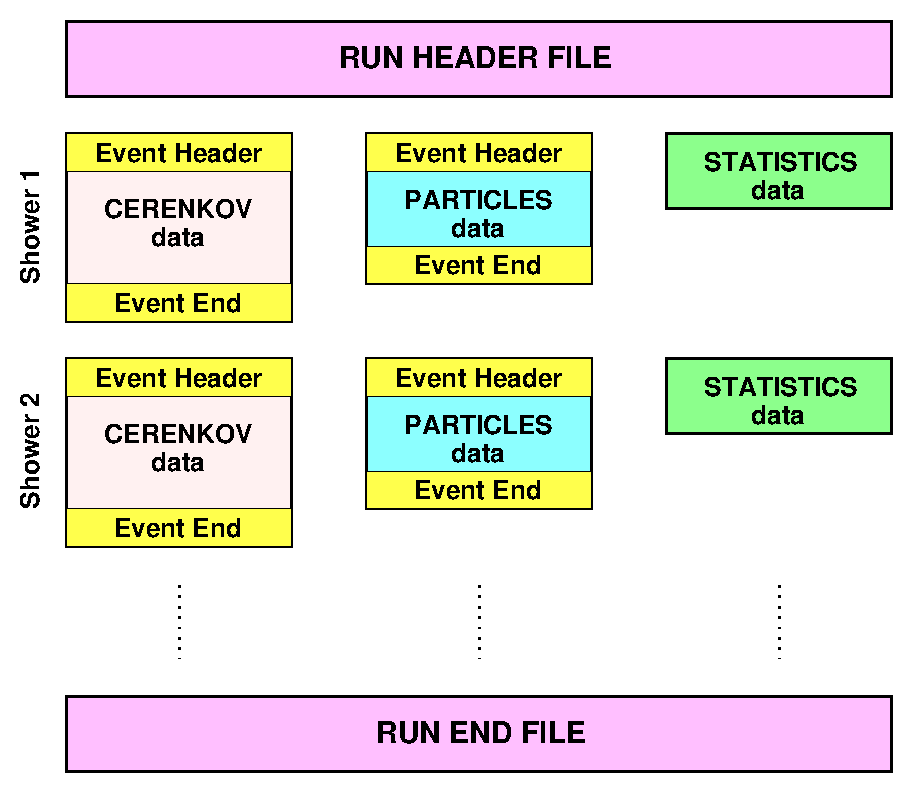
\epsfig{file=corsikastruc.eps,width=0.75\textwidth}
    \caption{Structure of the \CORSIKA output.}
    \label{fig:corsikastruc} 
  \end{center} 
\end{figure}
}

%%%%%%%%%%%%%%%%%%%%%%%%%%%%%%%%%%%%%%%%%%%%%%%%%%%%%%%%%%%%
\def\CORSIKAtableRH{
\begin{table}[p]
  \begin{center}
    \footnotesize
    \begin{tabular}{|r|l|}
\multicolumn{2}{c}{\bfseries Run header sub-block: (once per run)}\\
\hline
No. of word&Contents of word\\
\hline %%----------------------------------------
\hline %%----------------------------------------
1& `RUNH' \\
2& run number \\
3& date of begin run ( yymmdd ) \\
4&version of program \\
5& number of observation levels (maximum 10) \\
5+ $i$& height of level $i$ in cm\\
16 &slope of energy spectrum \\
17 &lower limit of energy range \\
18 &upper limit of energy range \\
19 &flag for EGS4 treatment of em. component \\
20 &flag for NKG treatment of em. component \\
21 &kin. energy cuto, for hadrons in GeV \\
22 &kin. energy cuto, for muons in GeV \\
23 &kin. energy cuto, for electrons in GeV \\
24 &energy cuto, for photons in GeV\\
\hline
\multicolumn{2}{|c|}{physical constants and interaction flags}\\
\hline
24+$i$ &C($i$), $i$ = 1,50 \\
74+$i$ &CC($i$), $i$ = 1,20 \\
94+$i$ &CKA($i$), $i$ = 1,40 \\
134+$i$& CETA($i$), $i$ = 1,5 \\
139+$i$& CSTRBA($i$),i = 1,11 \\
150+$i$& 0, $i$ = 1,4 (no longer used) \\
154+$i$& CAN($i$), $i$ = 1,50 \\
204+$i$& CANN($i$), $i$ = 1,50 \\
254+$i$& AATM($i$), $i$ = 1,5 \\
259+$i$& BATM($i$), $i$ = 1,5 \\
264+$i$& CATM($i$), $i$ = 1,5\\
270& NFLAIN (as real) \\
271& NFLDIF (as real) \\
272& NFLPI0+100$\times$NFLPIF (as real) \\
273& NFLCHE+100$\times$NFRAGM (as real)\\
\hline
    \end{tabular}
  \end{center}
  \caption{Structure of the run header sub-block}
  \label{tab:rh}
\end{table}
}

%%%%%%%%%%%%%%%%%%%%%%%%%%%%%%%%%%%%%%%%%%%%%%%%%%%%%%%%%%%%
\def\CORSIKAtableEHone{
\begin{table}[p]
  \begin{center}
    \footnotesize
    \begin{tabular}{|r|l|}
\multicolumn{2}{c}{\bfseries Event header sub-block: (once per event)}\\
\hline
No. of word&Contents of word\\
\hline %%----------------------------------------
\hline %%----------------------------------------
1& `EVTH'  \\
2& event number  \\
3& particle id (particle code or A$\times$ 100+Z for nuclei)  \\
4& total energy in GeV  \\
5& starting altitude in g=cm2  \\
6& number of first target if fixed  \\
7& z coordinate (height) of first interaction in cm  \\
8& px momentum in x direction in GeV  \\
9& py momentum in y direction in GeV  \\
10& pz momentum in -z direction in GeV \\
&(pz is positive for downward going particles)  \\
11& zenith angle $\theta$ in radian  \\
12& azimuth angle $\phi$ in radian  \\
13& number of different random number sequences (max. 10)  \\
11+3$\times$ $i$& integer seed of sequence $i$  \\
12+3$\times$ $i$& number of offset random calls ($\mathrm{mod} 10^6$) of sequence $i$  \\
13+3$\times$ $i$& number of offset random calls ($/10^6$) of sequence i \\
44& run number  \\
45& date of begin run (yymmdd)  \\
46& version of program  \\
47& number of observation levels  \\
47+$i$& height of level $i$ in cm \\
58& slope of energy spectrum  \\
59& lower limit of energy range in GeV  \\
60& upper limit of energy range in GeV  \\
61& cutoff for hadrons kinetic energy in GeV  \\
62& cutoff for muons kinetic energy in GeV  \\
63& cutoff for electrons kinetic energy in GeV  \\
64& cutoff for photons energy in GeV  \\
65& NFLAIN as a real number  \\
66& NFLDIF as a real number  \\
67& NFLPI0 as a real number  \\
68& NFLPIF as a real number  \\
69& NFLCHE as a real number  \\
70& NFRAGM as a real number  \\
71& x component of Earth's magnetic field in $\mu$T  \\
72& z component of Earth's magnetic field in $\mu$T  \\
73& flag for activating EGS4 as real number  \\
74& flag for activating NKG as real number \\
\hline
    \end{tabular}
  \end{center}
  \caption{Structure of event header sub-block.}
  \label{tab:eh1}
\end{table}
}

%%%%%%%%%%%%%%%%%%%%%%%%%%%%%%%%%%%%%%%%%%%%%%%%%%%%%%%%%%%%
\def\CORSIKAtableEHtwo{
\begin{table}[p]
  \begin{center}
    \footnotesize
    \begin{tabular}{|r|l|}
\multicolumn{2}{c}{\bfseries Event header sub-block: (continued)}\\
\hline
No. of word&Contents of word\\
\hline %%----------------------------------------
\hline %%----------------------------------------
75 &GHEISHA flag as real number                               \\
76 &VENUS flag as real number                                  \\
77 &CERENKOV flag as real number                               \\
78 &NEUTRINO flag as real number                               \\
79 &HORIZONT flag as real number                               \\
80 &computer flag (1=IBM, 2=Transputer, 3=DEC/UNIX,                              \\
&4=Macintosh, 5=VAX/VMS, 6=LINUX) as real number                               \\
81 &lower edge of $\theta$ interval (in $^\circ$)                               \\
82 &upper edge of $\theta$ interval (in $^\circ$)                               \\
83 &lower edge of OE interval (in $^\circ$)                               \\
84 &upper edge of OE interval (in $^\circ$)                               \\
85 &Cherenkov bunch size in the case of Cherenkov calculations                               \\
86 &number of Cherenkov detectors in x-direction                               \\
87 &number of Cherenkov detectors in y-direction                               \\
88 &grid spacing of Cherenkov detectors in x-direction in cm                               \\
89 &grid spacing of Cherenkov detectors in y-direction in cm                               \\
90 &length of each Cherenkov detector in x-direction in cm                               \\
91 &length of each Cherenkov detector in y-direction in cm                               \\
92 &Cherenkov output directed to particle output file (= 0.)                              \\
&or Cherenkov output file (= 1.)                                     \\
93 &angle (in rad) between array x-direction and magnetic north                               \\
94 &flag for additional muon information on particle output file                               \\
95 &step length factor for multiple scattering step length in EGS                               \\
96 &Cherenkov bandwidth lower end in nm \\
97 &Cherenkov bandwidth upper end in nm \\
98 &number $i$ of uses of each event \\
98+$i$& x coordinate of $i^{\mathrm{th}}$ core location for scattered events in cm \\
118+$i$& y coordinate of $i^{\mathrm{th}}$ core location for scattered events in cm\\
139 &SIBYLL interaction flag as real number \\
140 &SIBYLL cross section flag as real number \\
141 &QGSJET interaction flag as real number \\
142 &QGSJET cross section flag as real number \\
143 &DPMJET interaction flag as real number \\
144 &DPMJET cross section flag as real number \\
145 &VENUS cross section flag as real number \\
146 &muon multiple scattering flag (1.=Moli\`ere, 0.=Gauss) \\
147 &EFRCTHN energy fraction of thinning level \\
148 &NKG radial distribution range in cm \\
149...273 &not used\\
\hline
    \end{tabular}
  \end{center}
  \caption{Structure of event header sub-block (continued).}
  \label{tab:eh2}
\end{table}
}

%%%%%%%%%%%%%%%%%%%%%%%%%%%%%%%%%%%%%%%%%%%%%%%%%%%%%%%%%%%%
\def\CORSIKAtableEE{
\begin{table}[p]
  \begin{center}
    \footnotesize
    \begin{tabular}{|r|l|}
\multicolumn{2}{c}{\bfseries Event end sub-block}\\
\hline
No. of word&Contents of word\\
\hline %%----------------------------------------
\hline %%----------------------------------------
1 &`EVTE'  \\
2 &event number \\
&statistics for one shower :  \\
3 &weighted number of photons written to particle output file  \\
4 &weighted number of electrons written to particle output file  \\
5 &weighted number of hadrons written to particle output file  \\
6 &weighted number of muons written to particle output file  \\
7 &number of weighted particles written to particle output file PATAPE \\
&(This number includes also Cherenkov bunches, if Cherenkov output  \\
&is directed to PATAPE, but excludes additional muon information)  \\
&NKG output (if selected) :  \\
7+$i$&$i$= 1..21 lateral distribution in x direction for 1. level in \u{cm^2}\\  
28+$i$&$i$= 1..21 lateral distribution in y direction for 1. level in \u{cm^2}\\ 
49+$i$&$i$= 1..21 lateral distribution in xy direction for 1. level in \u{cm^2}\\
70+$i$&$i$= 1..21 lateral distribution in yx direction for 1. level in \u{cm^2}\\ 
91+$i$&$i$= 1..21 lateral distribution in x direction for 2. level in \u{cm^2}\\  
112+$i$&$i$= 1..21 lateral distribution in y direction for 2. level in \u{cm^2}\\ 
133+$i$&$i$= 1..21 lateral distribution in xy direction for 2. level in \u{cm^2}\\
154+$i$&$i$= 1..21 lateral distribution in yx direction for 2. level in \u{cm^2}\\
175+$i$&$i$= 1..10 electron number in steps of 100 \u{g/cm^2} \\ 
185+$i$&$i$= 1..10 age in steps of 100 \u{g/cm^2} \\ 
195+$i$&$i$= 1..10 distances for electron distribution in cm \\ 
205+$i$&$i$= 1..10 local age 1. level\\ 
215+$i$&$i$= 1..10 height of levels for electron numbers in \u{g/cm^2}\\  
225+$i$&$i$= 1..10 height of levels for electron numbers in cm \\ 
235+$i$&$i$= 1..10 distance bins for local age in cm \\ 
245+$i$&$i$= 1..10 local age 2. level \\ 
255+$i$&$i$= 1..6 parameters of longitudinal distribution of charged particles\\ 
262&$\chi^2$ per degree of freedom of fit to longitudinal distribution  \\
263..273&not used \\
\hline
    \end{tabular}
  \end{center}
  \caption{Structure of event end sub-block.}
  \label{tab:ee}
\end{table}
}

%%%%%%%%%%%%%%%%%%%%%%%%%%%%%%%%%%%%%%%%%%%%%%%%%%%%%%%%%%%%
\def\CORSIKAtableRE{
\begin{table}[p]
  \begin{center}
    \footnotesize
    \begin{tabular}{|r|l|}
\multicolumn{2}{c}{\bfseries Run end sub-block}\\
\hline
No. of word&Contents of word\\
\hline %%----------------------------------------
\hline %%----------------------------------------
1&`RUNE' \\
2&run number \\
3&number of events processed \\
4..273&not used yet\\
\hline
    \end{tabular}
  \end{center}
  \caption{Structure of run end sub-block.}
  \label{tab:re}
\end{table}
}

%%%%%%%%%%%%%%%%%%%%%%%%%%%%%%%%%%%%%%%%%%%%%%%%%%%%%%%%%%%%
\def\CORSIKAtablePART{
\begin{table}[p]
  \begin{center}
    \footnotesize
    \begin{tabular}{|r|l|}
\multicolumn{2}{c}{\bfseries Particle data sub-block : (up to 39 particles, 7 words each)}\\
\hline
No. of word&Contents of word \\
\hline %%----------------------------------------
\hline %%----------------------------------------
$7\times (n-1)+1$ &particle description \\
  &(part. id$\times$1000+ hadr. generation$\times$10+ no. of obs. level)  \\
$7\times (n-1)+2$ &px, momentum in x direction in GeV  \\
$7\times (n-1)+3$ &py, momentum in y direction in GeV  \\
$7\times (n-1)+4$ &pz, momentum in -z direction in GeV  \\
$7\times (n-1)+5$ &x coordinate in cm  \\
$7\times (n-1)+6$ &y coordinate in cm  \\
$7\times (n-1)+7$ &t time since first interaction in nsec \\
&(z coordinate in cm for additional muon information)  \\
\hline
\multicolumn{2}{|c|}{for n = 1 \ldots 39}\\
\multicolumn{2}{|c|}{last block may not be completely filled}\\
\hline
    \end{tabular}
  \end{center}
  \caption{Structure of particle data sub-block.}
  \label{tab:part}
\end{table}
}

%%%%%%%%%%%%%%%%%%%%%%%%%%%%%%%%%%%%%%%%%%%%%%%%%%%%%%%%%%%%
\def\CORSIKAtableCHER{
\begin{table}[p]
  \begin{center}
    \footnotesize
    \begin{tabular}{|r|l|}
\multicolumn{2}{c}{\bfseries Cherenkov photon data sub-block : (up to 39 photons, 7 words each)}\\
\hline
No. of word&Contents of word \\
\hline %%----------------------------------------
\hline %%----------------------------------------
$7\times (n-1)+1$ &j$\times$100000.+$\lambda$ \\
$7\times (n-1)+2$ &x coordinate in the obs.level, in cm\\
$7\times (n-1)+3$ &y coordinate in the obs.level, in cm\\
$7\times (n-1)+4$ &u direction cosine to x axis\\
$7\times (n-1)+5$ &v direction cosine to y axis\\
$7\times (n-1)+6$ &arrival time since first interaction in nsec\\
$7\times (n-1)+7$ &height of production of photon in cm\\
\hline
\multicolumn{2}{|c|}{for n = 1 \ldots 39}\\
\multicolumn{2}{|c|}{last block may not be completely filled}\\
\hline
    \end{tabular}
  \end{center}
  \caption{Structure of Cherenkov photon data sub-block. The value of 
    $j$ is defined as $j\equiv$number of the telescope which gave
    trigger (usually 1). We simulate with a bunch size (number of
    photons per sub-block) equal to 1.}
  \label{tab:cher}
\end{table}
}

%%%%%%%%%%%%%%%%%%%%%%%%%%%%%%%%%%%%%%%%%%%%%%%%%%%%%%%%%%%%
\def\CORSIKAtableSTA{
\begin{table}[p]
  \begin{center}
    \footnotesize
    \begin{tabular}{|r|l|}
\multicolumn{2}{c}{\bfseries Statistics data block}\\
\hline
No. of word&Contents of word \\
\hline %%----------------------------------------
\hline %%----------------------------------------
  1 \ldots 273 (273)& Event Header for this shower\\
274 \ldots 547 (273)&Event End for this shower\\
\hline
548&Time of the first photon stored in tape\\
549&Time of the last photon stored in tape\\
\hline
\multicolumn{2}{|c|}{for $i$ = 0 \ldots 9 $\longrightarrow$ 10 obs.levels}\\
\hline
550+$i\times 22$&Number of protons at obs.level $i$ \\
551+$i\times 22$&Number of antiprotons at obs.level $i$ \\
552+$i\times 22$&Number of neutrons at obs.level $i$ \\
553+$i\times 22$&Number of antineutrons at obs.level $i$ \\
554+$i\times 22$&Number of photons at obs.level $i$ \\
555+$i\times 22$&Number of electrons at obs.level $i$ \\
556+$i\times 22$&Number of positrons at obs.level $i$ \\
557+$i\times 22$&Number of neutrinos at obs.level $i$ \\
558+$i\times 22$&Number of $\mu^-$ at obs.level $i$ \\
559+$i\times 22$&Number of $\mu^+$ at obs.level $i$ \\
560+$i\times 22$&Number of $\pi^0$ at obs.level $i$ \\
561+$i\times 22$&Number of $\pi^-$ at obs.level $i$ \\
562+$i\times 22$&Number of $\pi^+$ at obs.level $i$ \\
563+$i\times 22$&Number of $K^0$ Long at obs.level $i$ \\
564+$i\times 22$&Number of $K^0$ Short  at obs.level $i$ \\
565+$i\times 22$&Number of $K^{*-}$  at obs.level $i$ \\
566+$i\times 22$&Number of $K^{*+}$  at obs.level $i$ \\
567+$i\times 22$&Number of strange Baryons at obs.level $i$ \\
568+$i\times 22$&Number of Deuterons at obs.level $i$ \\
579+$i\times 22$&Number of Tritons at obs.level $i$ \\
570+$i\times 22$&Number of $\alpha$ particles at obs.level $i$ \\
571+$i\times 22$&Number of other (strange) particles at obs.level $i$ \\
\hline
770&Number of Nucleons\\
771&Number of Pions   \\
772&Number of Etas    \\
773&Number of Kaons   \\
773&Number of strange Baryons\\
774&Number of Cherenkov photons from Electrons\\
775&Number of Cherenkov photons from Electrons\\
\hline
776&LPCT1 = 1 if Long.Distribution must be calculated\\
777&$N_{\mathrm{STEP}}$: Number of steps in the  Long.Distribution\\
778&$W_{\mathrm{STEP}}$: Width of the step in the  Long.Distribution\\
\hline
\multicolumn{2}{|c|}{\underline{\itshape Longitudinal distributions}}\\
\multicolumn{2}{|c|}{for $k$ = 0 \ldots 8 $\longrightarrow$ 9 species}\\
\multicolumn{2}{|c|}{$\gamma$,e$^+$,e$^-$,$\mu^-$,$\mu^+$,hadrons,charged
particles,nuclei and Cherenkov photons}\\
\multicolumn{2}{|c|}{and for $i$ = 0 \ldots $N_{\mathrm{STEP}}$}\\
\multicolumn{2}{|c|}{ $\longrightarrow$ $N_{\mathrm{STEP}}$ steps 
of $W_{\mathrm{STEP}}$}\\
\hline
779+$k\times N_{\mathrm{STEP}}+i$&Number of particles of specie
$k$ at depth $i\times W_{\mathrm{STEP}}$ g/cm$^2$ \\
\hline
    \end{tabular}
  \end{center}
  \caption{Structure of Statistics data block as saved in the
    \texttt{staXXXXXX} files.}
  \label{tab:sta}
\end{table}
}